\documentclass[a4paper, twoside]{report}
\usepackage{graphicx}
\DeclareGraphicsExtensions{.pdf,.png,.jpg}

\begin{document}
\chapter*{Building Gene Regulatory Network: experimental approach}
\section*{Introduction}

Developmental gene regulatory networks (dGRNs) plays a crucial role in the development of every single individual, especially multicellular. 
They regulate developmental processes not only during embryogenesis, but also affect post-embrionic morphogenetic processes like regeneration, asexual reproduction and growth.

GRN can be viewed as highly complicated network of protein-gene interactions. 
As a proteins in most of the cases act transcription factors (TFs). 
TFs are the proteins which has special DNA-binding motifs in their structure. 
This allows them to bind to regulatory elements in adjacent to gene regions (cis-regulatory modules) and regulate gene expression.
Depending on type of the interaction (activation/repression) there are can be several outcomes.
If TF binds to enchancer region, gene expression increase.
Opposite to that, if protein binds to silencer region then gene decrease its expression.
Also there can be more complicated types of interaction. 
For example protein could be insulator, enhancer-blocker or a barrier.
As a result most of the processes during development can be seen as complex network with lots of different gene-protein interactions.
Such networks usually illustrated using graphs.  
Nodes shows genes, TFs or signal molecules, edges illustrate types of interaction.
Such graphs in some cases reach vary big complexity.
As a consequense arise a questions: how can we reconstruct such networks? 
What kind of data should we use? 
And what are the potencial outcomes from reasearch of such gene interactions?

The purpose of this review was to demonstrate different approaches in building gene regulatory networks.
Special attention was paid to developmental GRNs.  

\section*{Developmental gene regulatory networks}

Term developmental gene regulatory networks (dGRNs) was first introduced by E. H. Davidson.
Usually this term refers to a GRN which preferentially consists of genes crucial for the development. 

\begin{figure}[h]
\center{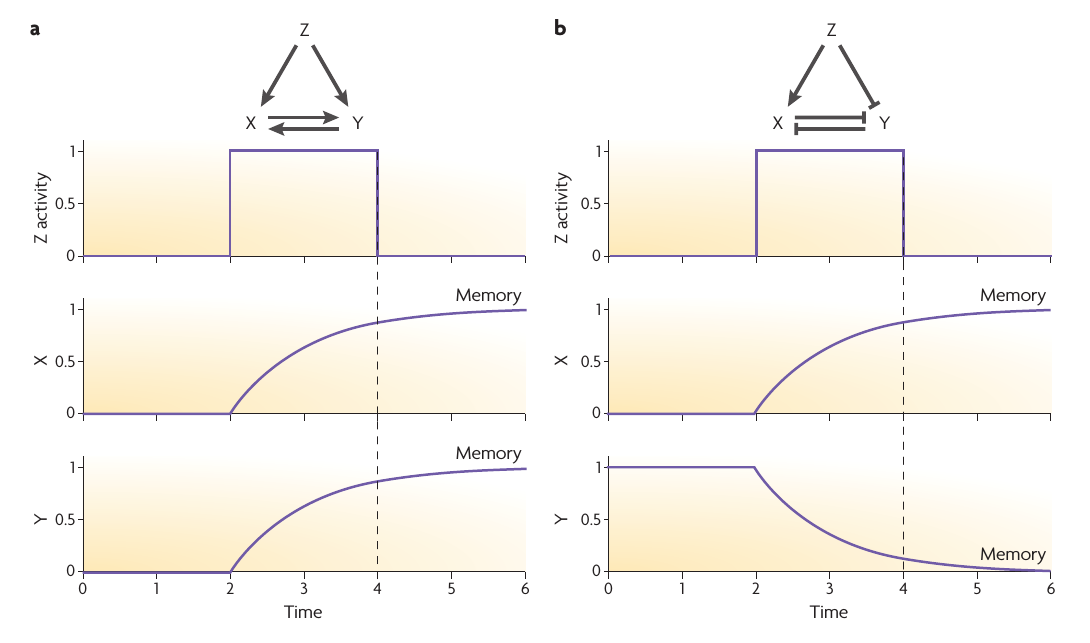
\includegraphics[width=1\linewidth]{fig_1}}
\caption{Two types of positive-feedback loops. Graph with curves represent activity (mRNA concentration) of the X,Y and Z genes. 
a | Network motifs with a double-positive-feedback loop.
b | Regulated feedback with a double-negative-feedback loop.}
\label{fig:fig_1}
\end{figure}

Developmental GRNs share lots of common features with other types of gene networks \cite{Alon2007}.
For example lots of networks typically has the same recurring regulation patterns as positive autoregulation (PAR), negative autoregulation (NAP), feedforward loops (FFLs) etc.
This common patterns called network motifs.
It is recurring circuits of interactions from which the gene networks are built.
Also usually GRNs have hierarchical structure \cite{Erwin2009}.
It means that those genes that control the initial stages of development are at the top of the hierarchy and those genes that execute the detailed functions of cell differentiation are at the periphery.
Consequently, changes in upstream genes have far larger effect than in downstream.
For example changes in gap genes in early development of \textit{Drosofila melanogaster} have more impact on final body plan than changes in genes which regulate eyes pigmentation.
There are lots of others similarities.
But at the same time developmental GRNs have their own characteristic features.

First of all, they tend to have longer cascades than some other GRNs.
It can be explained by the role of this cascades.
Often they require transduce signal through the whole process of development, through lots of cell generations.
That is why timescale of such process is very slow.
Sometimes it is one cell generation at each cascade step.
And that brings us to the second characteristic feature of developmental GRNs.

They can functioning even after input signal has vanished.
The signal can be inherited during cell division and subsequently be transduced to next cell generations.
In this case often used repressor cascades
Since they are more tolerant to concentration biases of signal molecule.

Such signal inheritance occures because of positive-feedback loops (PFLs).
PFL is a process in which two events are mutually reinforcing each other.
There are two kind of PFLs: double-positive loop and a double-negative loop (fig. 1).

In doble-positive-feedback loop (fig.1a) when signal molecule Z is activated, proteins X and Y begin to be produced. 
And after that X and Y develop self-sustained loop in which each molecule activate their partner.
After that even if Z is discarded (dashed line), loop A-B continue existinig.

In doble-negative-feedback loop (fig.2a), initially, there is a high concentration of Y and it represes X.
After Z is activated, X is produced and Y is repressed.
As a result after deactivation of Z (dashed line) signal is transduced by X.
Y at the same moment is discarded.
Thus, the feedback implements a memory.
And that is how dGRNs transduce signal after vanishing of signal input.

Because of these features study of dGRNs has several difficulties.
As we now understand in study of developmnent we always deal with dynamic biological systems.
That is why researcher have to monitor multiple time points.
Moreover he has to understand the start and the end point of studied process.

Next we discuss how solve such difficulties and try to review common technologies which is involved in GRN building.   

\section*{Experiment}

In order to build GRN related to any development process we need the following data:

\vspace{2mm}

1) What TFs or signal molecules are participate in the process? 

2) When does genes of those factors expresses? (Temporal expression)

3) Where does that happens? (Spatial expression)

4) And how they interact with each other?

\vspace{2mm}

We can distinguish two main approaches in building GRN. First is exprimental approch. In this way we predominantly operate experimental data (microarrays, qPCR, hybridisation \textit{in situ} etc). Second is computation approach or modeling GRN based on some descriptive and mathematical models using already generated data. In this review we will concentrate on first approach. In subsequent literature reviews we will cover second approach.

\subparagraph{Temporal expression}

\subparagraph{Spatial expression}

\subparagraph{Linkages}

\subparagraph{Validation}

\subparagraph{Visualisation}

\section*{Conslusion}


Therefore research of such a complex regulatory systems can shed more light on developmenatal processes and help in the curing of molecular genetic diseases associated with the violation of the networks.

\bibliographystyle{abbrv}
\bibliography{references}

\end{document}



